%#% extstart input preamble.tex
%
% This has been built from Memoir class
%             Author: Peter Wilson
%             Copyright 2001, 2002, 2003, 2004, 2008, 2009 Peter R. wilson
%
\listfiles
\documentclass[10pt,a4paper,extrafontsizes]{memoir}
\usepackage{comment}


% For (non-printing) notes  \PWnote{date}{text}
\newcommand{\PWnote}[2]{} 
\PWnote{2009/04/29}{Added fonttable to the used packages}
\PWnote{2009/08/19}{Made Part I a separate doc (memdesign.tex).}

% same
\newcommand{\LMnote}[2]{} 


\usepackage{memsty}
%%%%%%%%%%%%%%%%%%%%%%%%%%%%
\usepackage{titlepages}  % code of the example titlepages
\usepackage{memlays}     % extra layout diagrams
\usepackage{dpfloat}     % floats on facing pages
\usepackage{fonttable}[2009/04/01]   % font tables
%%%%\usepackage{xr-hyper} \externaldocument{memdesign} Doesn't work, 
%%%%                      Idea won't work in general for memman/memdesign
%%%%                      as at display time, who knows where everything
%%%%                      will be located on the individual's computer.
%%%%%%%%%%%%%%%%%%%%%%%%%%%%

%%%% Change section heading styles
%%%\memmansecheads

%%%% Use the built-in division styling
\headstyles{memman}

%%% ToC down to subsections
\settocdepth{subsection}
%%% Numbering down to subsections as well
\setsecnumdepth{subsection}

%%%% extra index for first lines
\makeindex[lines]


% this 'if' is used to determine whether we are compiling the memoir
% master in the subversion repository, or the public memman.tex
\newif\ifMASTER
\MASTERfalse
%\MASTERtrue

\ifMASTER

% add patch to fink, such that \AtEndFile still work
\makeatletter
\AtEndFile{fink.sty}{
  \typeout{patching fink} 
  \renewcommand{\InputIfFileExists}[2]{%
    \IfFileExists{##1}%
    {##2\@addtofilelist{##1}%
      \m@matbeginf{##1}%
      \fink@prepare{##1}%
      %\@@input \@filef@und
      \expandafter\fink@input%
      \expandafter\fink@restore\expandafter{\finkpath}%
     \m@matendf{##1}%
     \killm@matf{##1}}%
 }
}
\makeatother
% private package, not in circulation
% enables us to gather svn information on a single file basis
%\usepackage[filehooks]{svn-multi-private}
% use the current version
\usepackage[filehooks]{svn-multi}


% \svnidlong
% {}
% {$LastChangedDate: 2018-12-12 12:53:37 +0100 (Wed, 12 Dec 2018) $}
% {$LastChangedRevision: 622 $}
% {$LastChangedBy: daleif@math.au.dk $}



\makeatletter
\newcommand\addRevisionData{%
  \begin{picture}(0,0)%
    \put(0,-20){%
      \tiny%
      \expandafter\@ifmtarg\expandafter{\svnfiledate}{}{%
        \textit{\textcolor{darkgray}{Chapter last updated \svnfileyear/\svnfilemonth/\svnfileday
         \enspace (revision \svnfilerev)}}
     }%
    }%
  \end{picture}%
}
\makeatother

% we add this to the first page of each chapter

\makepagestyle{chapter}
\makeoddfoot{chapter}{\addRevisionData}{\thepage}{}
\makeevenfoot{chapter}{\addRevisionData}{\thepage}{}

\else
% disable svn info collecting
\newcommand\svnidlong[4]{}
\fi



%% end preamble
%%%%%%%%%%%%%%%%%%%%%%%%%%%%%%%%%%%%%%%%%%%%%%%%%%%%%%%
%#% extend

\usepackage[draft]{fixme}
\fxsetup{
  multiuser,
  marginface=\normalfont\tiny,
  innerlayout=noinline,
  layout=marginnote,
}
\usepackage{tikz,ragged2e}
\makeatletter
% extra feature, vadj=length kan flytte på fxnotes hvis de overlapper
\@fxdefinekey{layout}{vadj}{\def\marginnotevadjust{#1}}

% endnu mere ekstra feature, kræver tikz og calc tikz lib

\renewcommand*\FXLayoutMarginNote[3]{%
  \tikz[overlay,remember picture]\coordinate (A) at (0,0);%
  \marginnote[%
    \RaggedLeft%
    \rlap{\tikz[overlay,remember picture]\coordinate(C) at (0,0);}%
    \@fxuseface{margin}%
    \@fxtextstd{#1}{#2}{#3}%
    {\tikz[overlay,remember picture,ultra thin,cyan]\draw(A) -| ++(0,-2pt) -|(C);}%
  ]{%
    \RaggedRight%
    \tikz[overlay,remember picture]\coordinate(B) at (0,0);%
    \@fxuseface{margin}%
    \@fxtextstd{#1}{#2}{#3}%
    \tikz[overlay,remember picture,ultra thin,cyan]\draw(A) -| ++(0,-2pt) -|(B);%
  }%
}
\makeatother



\begin{document}


%#% extstart input intro.tex





%\tightlists
\firmlists
\midsloppy
\raggedbottom
\chapterstyle{demo3}

%%%%%%%%%%%%%%%%%%%%%%%%%%%%%%%%%%%%%%%%%%%%%%%%%%%%%%%


\ProvidesFile{memnoidxnum}[2009/04/30  some index entries for memman]
\newcommand*{\idxat}{\index{@?\texttt{@}|noidxnum}} \idxat
%%\index{@?\texttt{@}|noidxnum}
\index{argument|noidxnum}
%%\index{array|noidxnum}
\index{cardinal|noidxnum}
\index{centering|noidxnum}
%%\index{chapterstyle|noidxnum}
%%\index{counter|noidxnum}
\index{default|noidxnum}
\index{division|noidxnum}
\index{division!sectional|seealso{subhead}}
\index{double column|noidxnum}
\index{endnote!mark|seealso{reference mark}}
\index{environment|noidxnum}
\index{error message|noidxnum}
\index{figures|noidxnum}
%%\index{file|noidxnum}
\index{font characteristic|noidxnum}
\index{footnote!mark|seealso{reference mark}}
\index{footnotes|noidxnum}
\index{frame|noidxnum}
\index{framed|noidxnum}
\index{full stop|seealso{period}}
\index{hanging|noidxnum}
\index{headstyles|noidxnum}
%%\index{horizontal|noidxnum}
\index{Hurenkinder|see{widow}}
\index{interlinear space|see{leading}}
\index{keyword|noidxnum}
%%\index{label|noidxnum}
\index{LaTeX?\ltx|noidxnum}
%%\index{length|noidxnum}
\index{line|noidxnum}
\index{line too long|see{overfull lines}}
\index{lining|noidxnum}
%%\index{list|noidxnum}
\index{lowercase|noidxnum}
\index{MakeIndex?\Pmakeindex|noidxnum}
\index{margin!spine|seealso{inner}}
\index{margin!inner|seealso{spine}}
\index{margin!foredge?\foredge|seealso{outer}}
\index{margin!outer|seealso{\foredge}}
\index{margin!upper|seealso{top}}
\index{margin!top|seealso{upper}}
\index{math|noidxnum}
%%\index{memoir class|noidxnum}
\index{minipage|noidxnum}
\index{name|noidxnum}
\index{named|noidxnum}
\index{new|noidxnum}
%%\index{number|noidxnum}
\index{numeric|noidxnum}
\index{old-style|noidxnum}
\index{option|noidxnum}
\index{ordinal|noidxnum}
\index{outline|noidxnum}
\index{package|noidxnum}
\index{page break|noidxnum}
%%\index{pagestyle|noidxnum}
\index{paragraph break|noidxnum}
\index{period|seealso{full stop}}
\index{poem|noidxnum}
\index{program|noidxnum}
\index{ranging|noidxnum}
\index{reference|noidxnum}
\index{reference mark|seealso{endnote mark, footnote mark}}
\index{representation|noidxnum}
\index{rule|noidxnum}
\index{ruled|noidxnum}
%%\index{section|noidxnum}
\index{Schusterjungen|see{orphan}}
\index{section|seealso{subhead}}
\index{sectional division|seealso{subhead}}
\index{single column|noidxnum}
\index{size|noidxnum}
\index{space|noidxnum}
\index{space!double|see(double spacing)}
\index{space!between lines|see{leading}}
\index{stanza|noidxnum}
%%\index{subfloat|noidxnum}
\index{TeX?\tx|noidxnum}
\index{text|noidxnum}
\index{titling|noidxnum}
\index{trim|noidxnum}
%%\index{type size|noidxnum}
\index{vertical|noidxnum}
\index{warning|noidxnum}
\index{write|noidxnum}
%%\index{XeTeX?\xetx|noidxnum}

%%%%%%%% Deleted the font indexing (now done as typefaces) 2009/04/30

\begin{comment}
\index{table of contents|see{ToC}}
\index{list!of figures|see{LoF}}
\index{figure!list of|see{LoF}}
\index{list!of tables|see{LoT}}
\index{table!list of|see{LoT}}
\index{marginal note|see{marginalia}}
\index{footnote!in title|see{thanks}}
\index{illustration|seealso{float, figure}}
\index{figure|seealso{float}}
\index{table|seealso{float}}
\index{chapter!style|see{chapterstyle}}
\index{chapter!heading|see{heading}}
\index{page!style|see{pagestyle}}
\index{part!heading|see{heading}}
\end{comment}

\begin{comment}

%%%% deleted the \nocites
%
\index{anonymous division|see{division}}
\index{array|seealso{tabular}}
%
\index{Berne Convention|see{copyright}}
\index{blank page|see{page}}
\index{Buenes Aires Convention|see{copyright}}
\index{box!rule|seealso{rule}}
%
\index{chapter|seealso{division}}
\index{chapter!style|see{chapterstyle}}
\index{command|seealso{declaration, macro}}
\index{comptexttex?\texttt{comp.text.tex} newsgroup|see{\ctt}}
\index{Comprehensive TeX Archive Network?\cTeXan|see{\ctan}}
\index{contents list|see{ToC}}
\index{counter representation!Alph tt?\texttt{Alph}|see{\texttt{Alph}}}
\index{counter representation!alph tt?\texttt{alph}|see{\texttt{alph}}}
\index{counter representation!arabic tt?\texttt{arabic}|see{\texttt{arabic}}}
\index{counter representation!Roman tt?\texttt{Roman}|see{\texttt{Roman}}}
\index{counter representation!roman tt?\texttt{roman}|see{\texttt{roman}}}
\index{counter representation!fnsymbol tt?\texttt{fnsymbol}|see{\texttt{fnsymbol}}}
\index{cross reference|seealso{reference}}
%
\index{descriptive list|see{list}}
\index{display math|see{math}}
\index{display mode|see{display}}
\index{division|seealso{heading}}
%
\index{electronic book|see{ebook}}
\index{enumerated list|see{list}}
%
\index{figure!list of|see{LoF}}
\index{figure|seealso{float}}
\index{float!numbered captioning|see{caption}}
\index{float!unnumbered captioning|see{legend}}
\index{font characteristic!weight|see{series}}
%
\index{file|seealso{stream}}
\index{footnote!in title|see{thanks}}
\index{fragile command|seealso{protect}}
\index{free tabular|seealso{tabular}}
%
\index{header|seealso{running header}}
\index{heading|seealso{division}}
%
\index{illustration|seealso{float, figure}}
\index{inline math|see{math}}
\index{International Standard Book Number|see{ISBN}}
\index{itemized list|see{list}}
%
\index{label|seealso{reference}}
\index{left-to-right|see{LR}}
\index{list!new list of|see{list of, new}}
\index{list!of contents|see{ToC}}
\index{list!of figures|see{LoF}}
\index{list!of tables|see{LoT}}
\index{list of!contents|see{ToC}}
\index{list of!figures|see{LoF}}
\index{list of!tables|see{LoT}}
\index{LoF|seealso{ToC}}
\index{LoT|seealso{ToC}}
\index{log-like function|see{function}}
%
\index{macro|seealso{command}}
\index{margin note|seealso{marginalia}}
\index{marginalia|seealso{marginal note, side note, sidebar}}
%
\index{named division|see{division}}
%
\index{page!of floats|see{float, page}}
\index{page!start new|see{start new page}}
\index{page!style|see{pagestyle}}
\index{paragraph|seealso{division}}
\index{part|seealso{division}}
\index{picture object!Bezier curve|see{Bezier curve}}
\index{picture object!circle|see{circle}}
\index{picture object!line|see{line}}
\index{picture object!oval|see{box, rounded}}
\index{picture object!vector|see{vector}}
\index{poem|see{verse}}
\index{poetry|see{verse}}
\index{print run|see{impression}}
\index{protect|seealso{fragile command}}
%
\index{recto|seealso{odd page}}
\index{reference|seealso{label}}
\index{river|see{white space}}
\index{rivulet|see{white space}}
\index{running footer|see{footer}}
\index{running header|seealso{header}}
%
\index{section|seealso{division}}
\index{side note|seealso{marginalia}}
\index{sidebar|seealso{marginalia}}
\index{stanza|seealso{verse}}
\index{stanza!line number|see{line number}}
\index{subparagraph|seealso{division}}
\index{subsection|seealso{division}}
\index{subsubsection|seealso{division}}
%
\index{table of contents|see{ToC}}
\index{table!list of|see{LoT}}
\index{table|seealso{float}}
\index{tabular|seealso{array}}
\index{tabular!free|see{free tabular}}
\index{tabulation|see{tabular}}\
\index{TeX Users Group?\TeXUG|see{\tug}}
\index{textblock|see{typeblock}}
%
\index{Universal Copyright Convention|see{copyright}}
%
\index{verbatim!line number|see{line number}}
\index{verse|seealso{stanza}}
\index{verse!title|see{poem title}}
\index{verse!line number|see{line number}}
\index{verso|seealso{even page}}
\index{visual markup|see{visual design}}
%
\index{x coordinate|see{coordinate}}
%
\index{y coordinate|see{coordinate}}
%
%


\end{comment}

\endinput



\frontmatter
\pagestyle{empty}


% title page
\vspace*{\fill}
\begin{center}
\HUGE\textsf{The Stellar Command Module}\par
\end{center}
\begin{center}
\LARGE\textsf{for}\par
\end{center}
\begin{center}
\HUGE\textsf{Integrating Astronomy and Art}\par
\end{center}

\begin{center}
\Huge\textsf{User Guide}\par
\end{center}
\begin{center}
\LARGE\textsf{Angelo Fraietta}\par
\bigskip
\LARGE\textsf{University of New South Wales}\par
%\normalsize\textsf{Maintained by Angelo Fraietta}\par
\medskip

\end{center}
\vspace*{\fill}
\def\THP{T\kern-0.2em H\kern-0.4em P}%   OK for CMR
\def\THP{T\kern-0.15em H\kern-0.3em P}%   OK for Palatino
\newcommand*{\THPress}{The Herries Press}%
\begin{center}

%\includegraphics[width=\droptitle]{anvil2.mps}
\setlength{\droptitle}{0pt}%
\end{center}
\clearpage

\PWnote{2009/06/26}{Updated the copyright page for 9th impression}
% copyright page
\begingroup
\footnotesize
\setlength{\parindent}{0pt}
\setlength{\parskip}{\baselineskip}


\begin{tabular}{@{} l l}
  \textcopyright{} 2018\:---\:2019 &Angelo Fraietta \\
\end{tabular}


All rights reserved



\begin{center}
\begin{tabular}{ll}
First edition:                        & 6 June 2019 \\

\end{tabular}
\end{center}
\ifMASTER
Manual last changed \svnyear/\svnmonth/\svnday
\fi

\endgroup

\clearpage

\pagestyle{headings}
%%%%\pagestyle{Ruled}

\setupshorttoc
\tableofcontents
\clearpage
\setupparasubsecs
\setupmaintoc

\begingroup

% important point here: We need \endlineshar=-1 here for the inline
% list of subsections. Why? Beacause we have subsection subsubsection
% subsection, and under hyperref running the l@subsubsection for
% subsubsection, which typesets nothing, ruins our \ignorespaces in
% our redefinition of \l@subsection (it cannot see and ignore the space after the
% \contentsline line for subsubsection). Easiest solution: use
% change \endlinechar
%
% Special thanks to David Carlisle in the tex.stackexchange.com chat
% for suggesting it


\endlinechar=-1


\tableofcontents

\endgroup


\setlength{\unitlength}{1pt}
\clearpage
\listoffigures
\clearpage
\listoftables
\clearpage
\listofegresults

%#% extend


%#% extstart include preface.tex
%\chapter{Foreword}

\svnidlong
{$Ignore: $}
{$LastChangedDate: 2014-11-05 16:28:11 +0100 (Wed, 05 Nov 2014) $}
{$LastChangedRevision: 501 $}
{$LastChangedBy: daleif $}

\chapter{Preface}
    
    \textit{Stellar Command} is a software system that integrates \textit{Stellarium} planetarium software with online astronomical data acquisition through \textit{VizieR} database of astronomical catalogues \cite{ochsenbein2000vizier}. Stellar Command can be used as an interface mechanism for correlating music and sound generation, allowing Stellarium to be used as both a direct input interface for performance or composition, and as a remotely controlled derivative multimedia display output.   

	I hope you will have as much fun creating musical works with it as much as I have.
{\raggedleft{\scshape ngelo Fraietta} \\ Newcastle, AU \\ June 2019\par}


%#% extend

%#% extstart include intro-8.tex

\svnidlong
{$Ignore: $}
{$LastChangedDate: 2015-04-22 17:17:51 +0200 (Wed, 22 Apr 2015) $}
{$LastChangedRevision: 527 $}
{$LastChangedBy: daleif $}

\chapter{Introduction}
    Musical composition and performance inspired or based on astronomy has been used in many cultures for millennia, with many civilizations creating songs and dances based on the astronomical calendar to reinforce the tracking of seasonal activities; such as planting and harvesting of crops, times of trade, and religious or cultural practices \cite{ruggles2015handbook, deMello2015, Lima2015}.  More recently, composers  have used scientific data obtained from individual stars to generate sounds and have created compositions directly correlated to that data \cite{fraietta2014musical, BriightSyzygy}. 

The advancement of computing power has made the availability of planetarium software for both desktop and mobile platforms very accessible to many people. These software packages are not only used for scientific and research activities; such as astronomy, education and general stargazing; they have also been used by artists in presenting multimedia artworks and installations \cite{zotti2017skyscape,tuveri2013controlling}. 

Many composers have used the cosmos as inspiration or stimulus to their works, with many using scientific observations or data as input \cite{fraknoi2008music, fraietta2014musical}. The \textit{Quadrivium} linked astronomy, mathematics, geometry and music as a standard part of classical education up until the renaissance \cite{lundy2010quadrivium}. Composers have been mapping mathematics and geometry to music since antiquity \cite{james1995music, assayag2002mathematics}. Kepler stated ``The heavenly motions are nothing but a continuous song for several voices, to be perceived by the intellect, not by the ear; a music which, through discordant tensions, through syncopations and cadenzas as it were, progresses toward certain pre designed six-voiced cadences, and thereby sets landmarks in the immeasurable flow of time." \cite[cited in  ~286]{RojersRuffKepler}. This notion inspired Rogers and Ruff to compose \textit{The Harmony of the World} (1979), describing their work as ``A Realization for the Ear" \cite [p. 286]{RojersRuffKepler} of Johannes Kepler's Astronomical Data from Harmonices Mundi 1619.
More recently, composers have used measurements from online databases as inputs to automata or as stimulus to performers. 

Nick Ryan developed a musical instrument called \textit{Machine 9} that uses the location of 27,000 pieces of space junk as input to an automaton \cite{spaceDebrisNewScientist}. 
The instrument is a large cylindrical phonograph that maps space debris to sound as it directly passes overhead. Each groove on the cylinder is associated with a catalogued piece of space debris \cite{spaceDebrisYoutube}. The system accesses publicly available databases that provides the telemetry data of space debris, which is then modelled in real-time. When the telemetry data indicates that one of catalogued items is overhead, the machine locates one of the grooves on the cylinder and plays a mapped sound mechanically through a record-player type stylus. 

Another system based on astronomical catalogues was the author's own musical composition and performance interface using naked eye and binocular astronomy \cite{fraietta2014musical}. A specific star was determined by calculating its azimuth and height above the horizon--known as its \textit {altitude}--using  accelerometer and magnetometer sensors, and calculating the exact location of the star on the celestial sphere using the sensor data, time and geographical location of the observer. This calculation returns the star's \textit{right ascension (RA)}, which is based on its azimuth at Greenwich Meantime at the vernal equinox,  and its \textit{declination (Dec.)}, which is the stars north-south position at the same time \cite{duffett2011practical, fraietta2014musical}. The resultant RA and Dec. are added as input to the VizieR database of online catalogues, returning data about stars--such as brightness and colour--within the defined radius. Various works were created using this interface. In one performance, which was  conducted in conjunction with the Newcastle Astronomical Society on one of their field viewing nights, members of the  public were enticed into viewing the night sky through high powered binoculars, while the sound generated, which was  based on data from the stars they were viewing, was played through loudspeakers on the field \cite{fraietta_segue}. 
Another set of performances was conducted with an improvising ensemble that featured various astronomical photos displayed as a slide show where the astronomical data was mapped as MIDI and functioned as inspirational impetus for the performers \cite{BriightSyzygy}. 

Although both systems are innovative and impressive, they have identifiable boundaries. First, Machine 9 exists as an installation piece using unique piece of specialised hardware \cite{spaceDebrisYoutube}.  Furthermore, a publicly available API to convert the space debris to a musical transmission protocol like MIDI or OSC \cite{wright1997open} is not yet available for the wider computer music community. Secondly, although the binocular display has an awesome display--the actual night sky--``few people ventured outside to the astronomical equipment"\cite[p. ~50]{fraietta2014musical} because they were required to leave the room to look through binoculars while the ensemble played in a room. Furthermore, the work is severely bound by weather conditions and a clear view of the sky. In one of the performances, ``the sky was completely covered with cloud and it rained, so there was nothing to see through the binoculars. The audience, however, enjoyed the ensemble performance with the NASA image slide show with samples fed from stored star tables."\cite[p. ~50]{fraietta2014musical}.  This weather constraint inspired the author to use planetarium software as the input and display mechanism as an alternative to binoculars.  

Stellar Command enables composers to access astronomical data as input to their software using a common API.  It also enables them to provide the audience an impressive planetarium software display that runs on a laptop computer without requiring the audience to leave the room. Furthermore, it facilitates creation of interactive celestial based installations. Stellar Command is available as open source software through GitHub \cite{fraiettaSTELLARCOMMAND}.

\chapter{Background}
\section{Stellarium}
Stellarium is a software program designed to enable people to create a virtual planetarium using their home computer \cite{zottistellarium}. It runs on Windows, OSX and Linux/Unix, including Raspberry Pi \cite[p.~6]{zottistellarium}.  Stellarium calculates positions of the Sun, moon, stars and planets based on the time and location defined by the user, and renders them to the display.  Stellarium is used by both amateur and professional astronomers, and is used by the  European Organisation for Astronomical Research in the Southern Hemisphere to facilitate distribution and sharing of visual data among scientists \cite{berglund2008using}. Stellarium has a very high quality graphical display, supporting spherical mirror projection that can be used with a dome \cite{mc2009touring} and is used in many schools and museums because it is both scientifically accurate and visually engaging \cite{berglund2008using}.  Moreover, Stellarium can display constellations from several different cultures and has labels translated to more than 40 languages, making Stellarium both culturally aware and inclusive \cite{berglund2008using}. 
For example,  Figures~\ref{fig:WesternCrux} and ~\ref{fig:TukanoTortoise} display the same area of sky, however the first presents the constellations using the western sky lore while the latter presents them in the Tukano sky lore\footnote{The Tukano tribes are indigenous peoples of the northwestern region of Brazil \cite{KnoblochFrancis1976TTIA}.} \cite{reichel1976cosmology}. A comparison reveals that \textit{Scorpius} and \textit{Crux} are referred to as the \textit{Fer-de-lance} and the \textit{Tortoise}. This feature can make Stellarium an extremely useful tool in facilitating multimedia presentations for ethnomusicogy or composing in non-western contexts.

\begin{figure}[htbp]
	\centering
	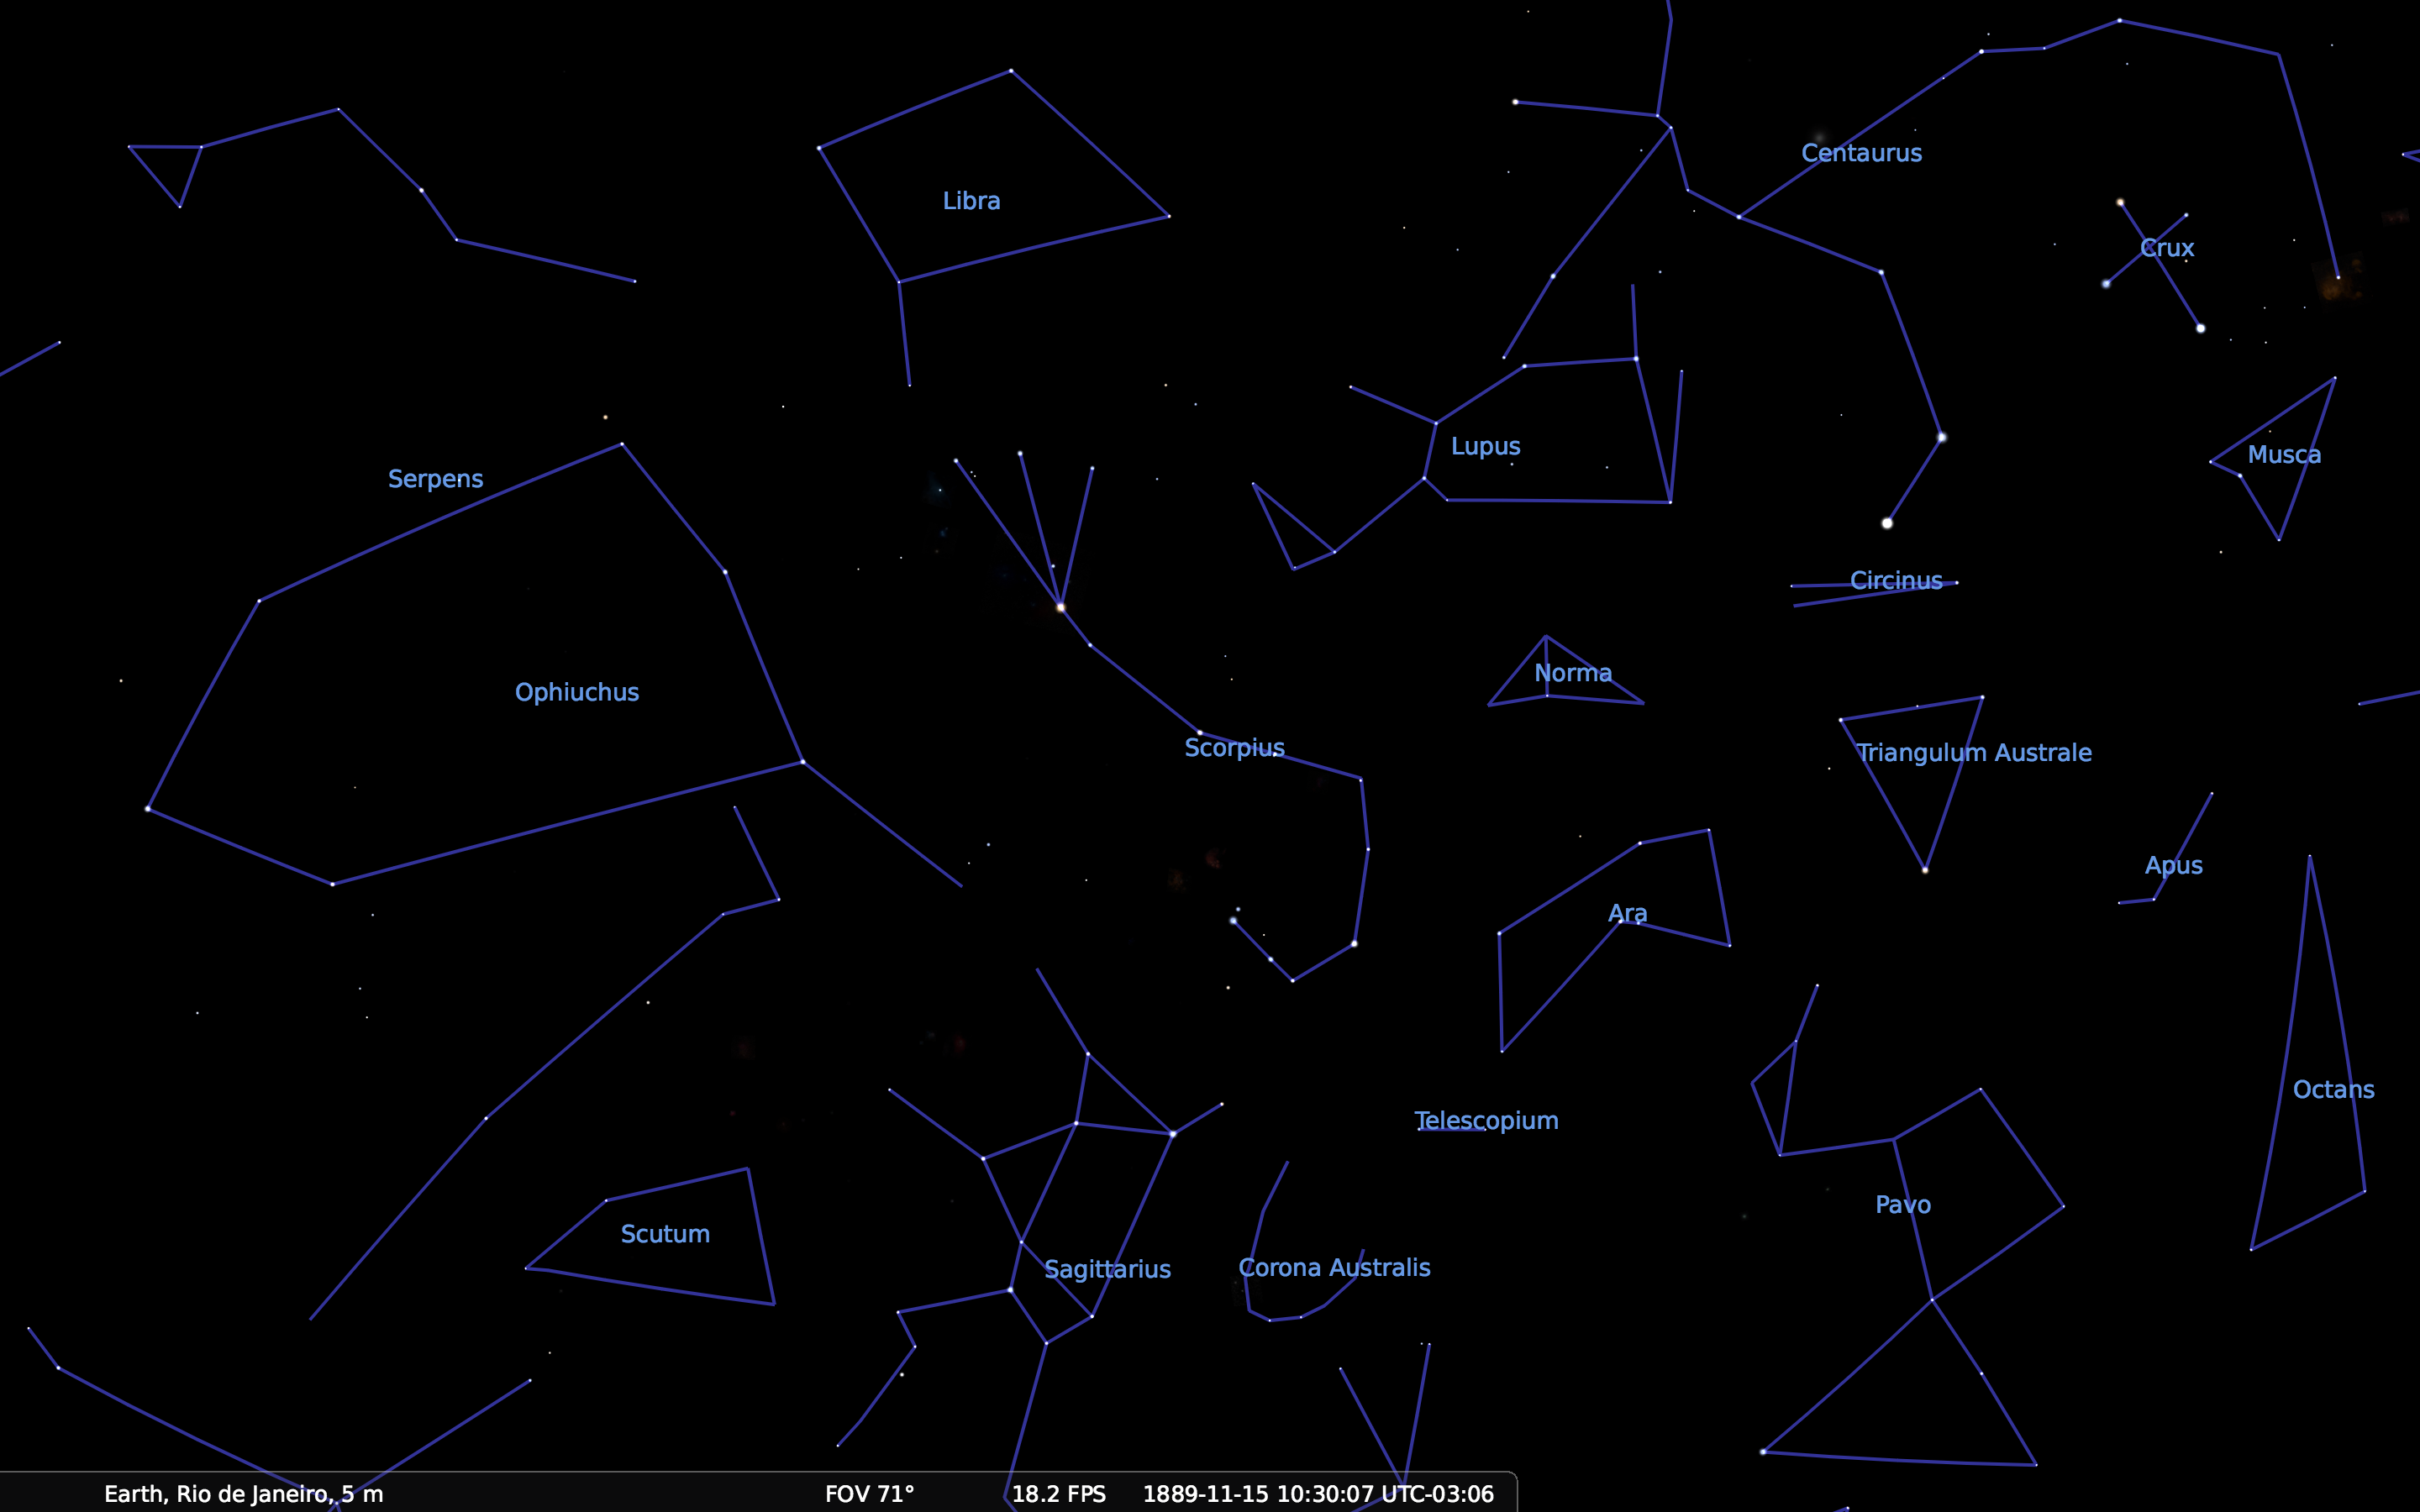
\includegraphics[width=1\columnwidth]{WesternCrux}
	\caption{Constellations displayed in Western sky lore.}
	\label{fig:WesternCrux}
\end{figure}

\begin{figure}[htbp]
	\centering
	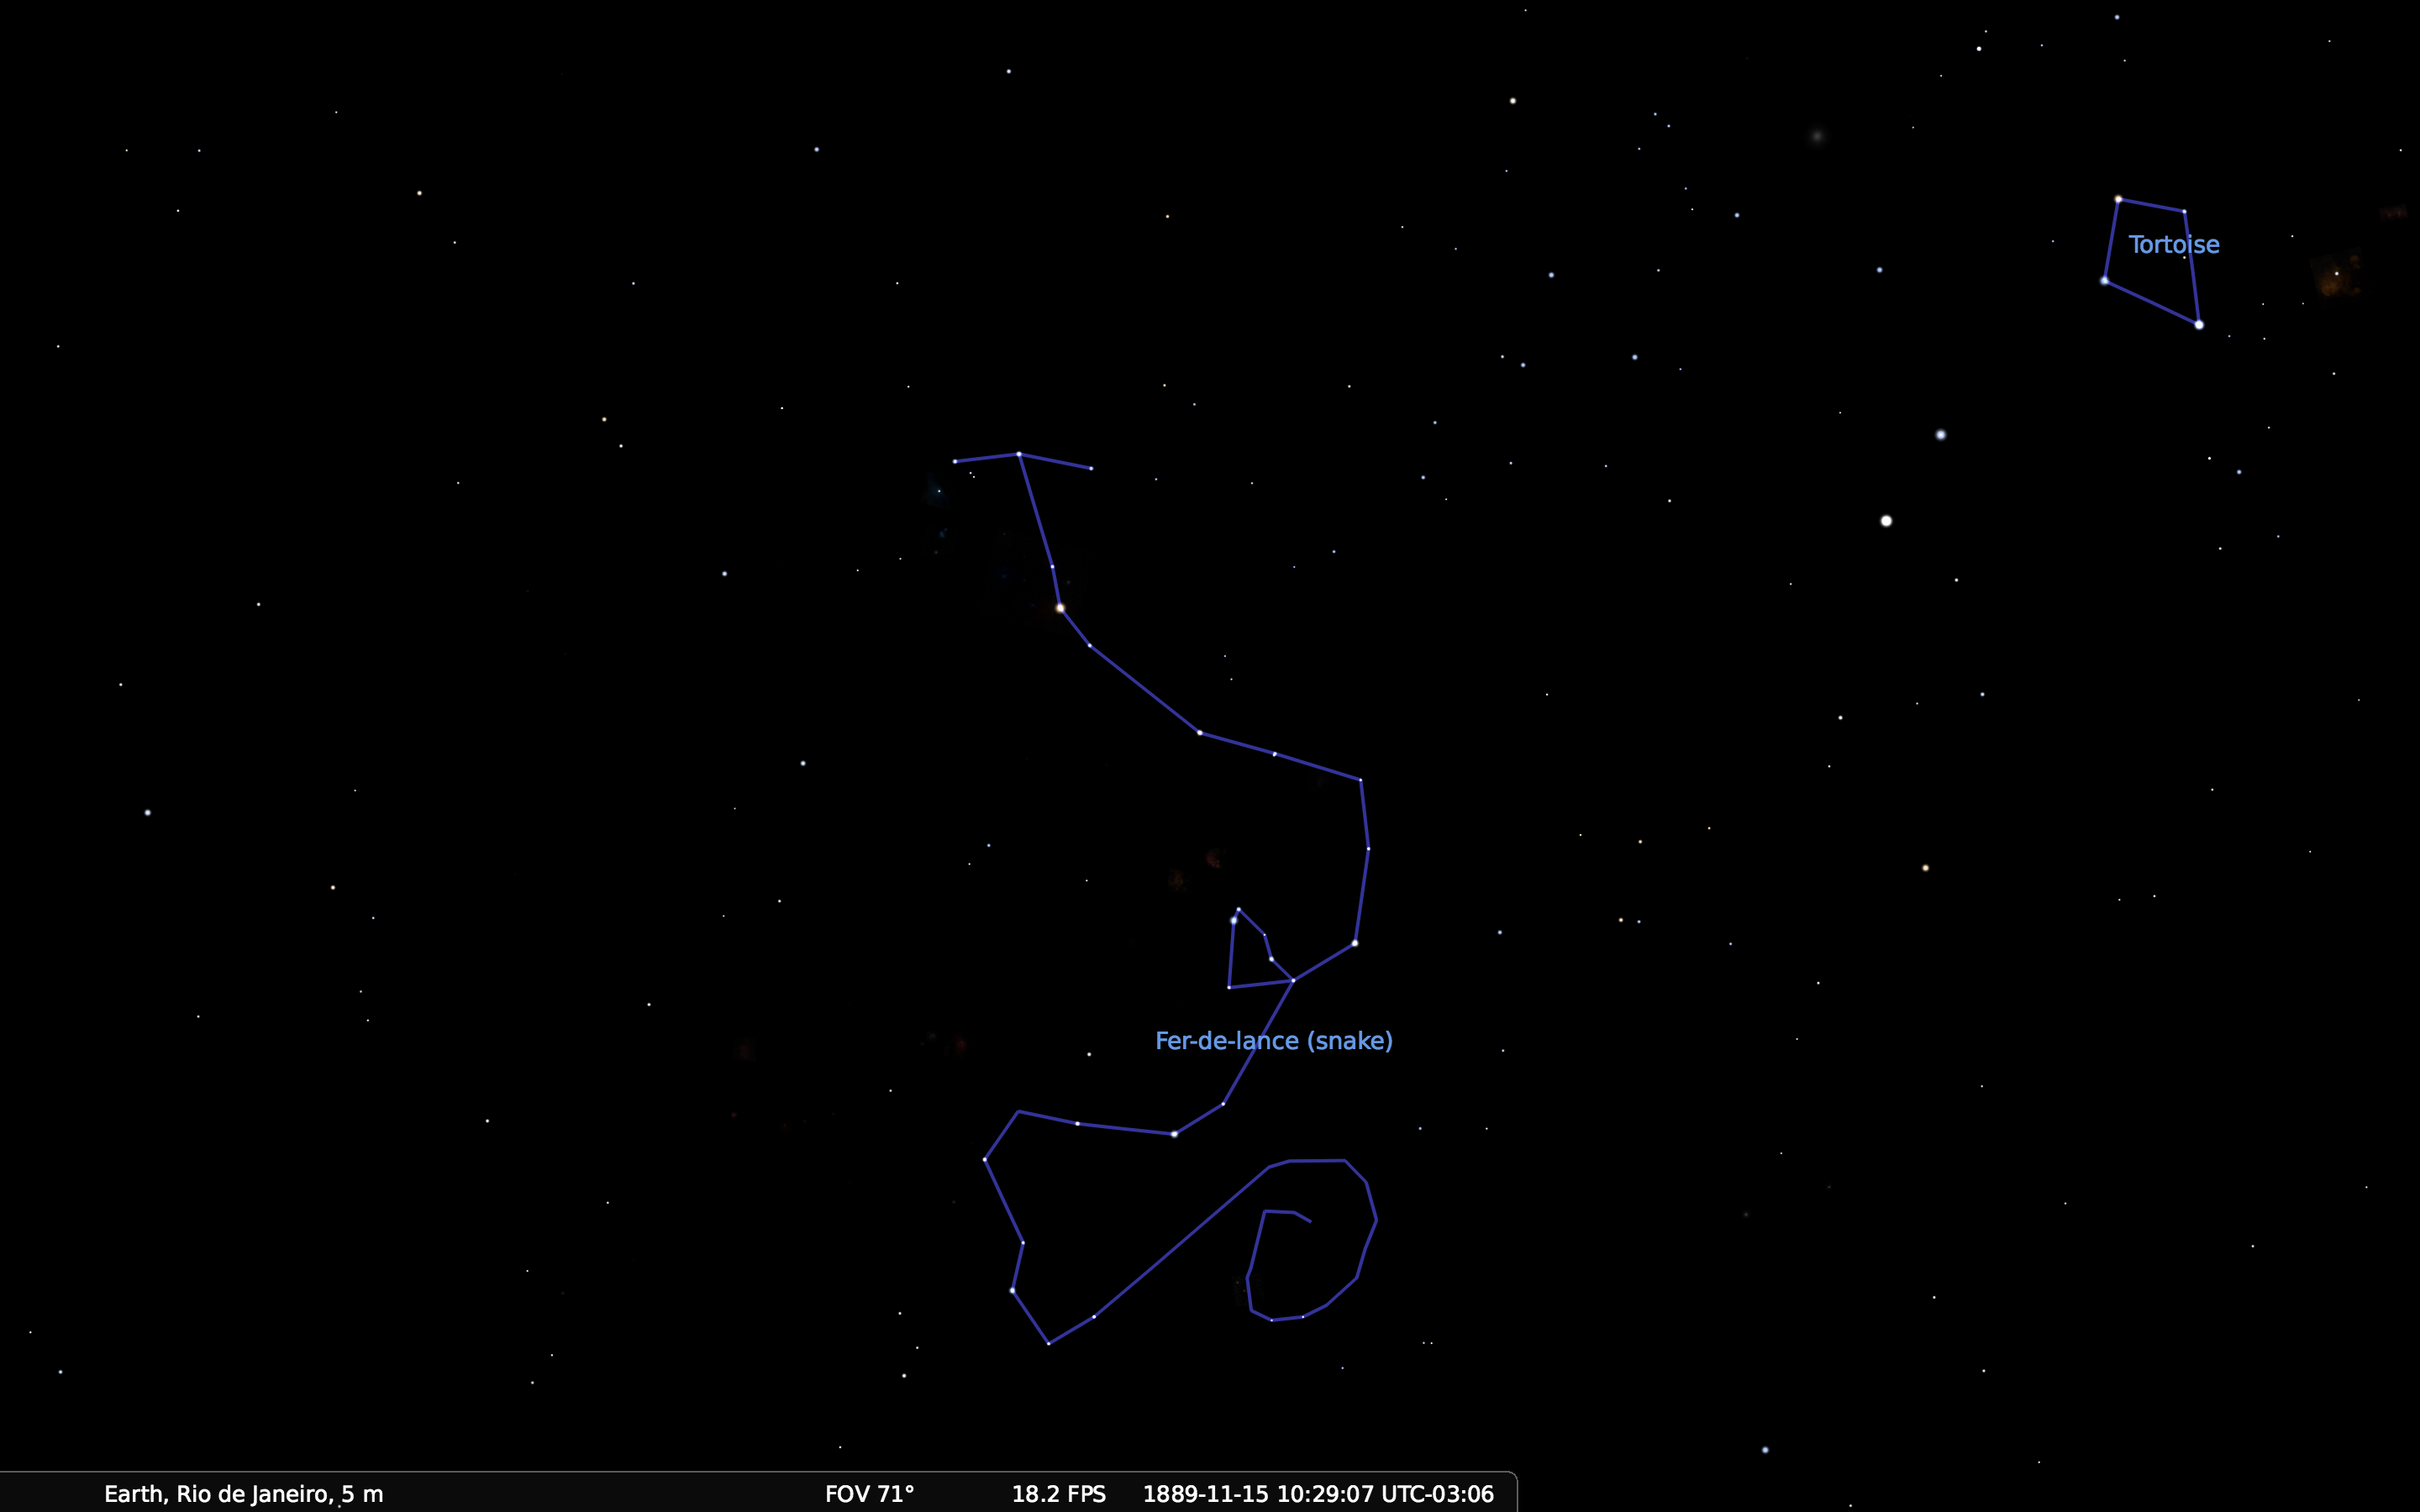
\includegraphics[width=1\columnwidth]{TukanoTortoise}
	\caption{Constellations displayed in Tukano sky lore.}
	\label{fig:TukanoTortoise}
\end{figure}

Many astronomers use Stellarium to display a prediction of the sky for a future time, such as organising a viewing night or planning an astro-photography session \cite{ashley2015computers}. Archaeoastronomers  also use the feature to generate an astronomical display from a location for a period sometime in the past \cite{zotti2014towards}. Also, the landscape feature facilitates a connection between  landscape and  skyscape, so one can map the sky against a landscape for research or aesthetics \cite{zotti2017skyscape}.

Stellarium scripts are written in ECMAScript, also known as Javascript, and enables the programmer to generate and run an automated astronomy presentation, facilitating  automation of all the functionality of Stellarium  \cite{zottistellarium}. 

Stellarium has a Remote Control plugin that enables third party programs to communicate with Stellarium via a REST client. This feature was used by the author to create an interactive spacecraft game using a sonic ball as a preliminary test of Stellarium's viability as a responsive performance interface \cite{fraiettaLAC2019}. The plugin also allows clients to query the status of Stellarium, including the area of sky currently being displayed.  The exact celestial vector and field of view displayed are used as the input to the VizieR server in order to obtain data about stars in that location.

\section{VizieR}
VizieR is an online database of high quality astronomical catalogues collected by the Centre de Donn\'ees astronomiques de Strasbourg (CDS), one of whose main goals  ``is to promote the usage of the reliable astronomical catalogues to the astronomical community" \cite[p.~25]{ochsenbein2000vizier}. One of the ways CDS ensures the reliability of their archives and catalogues is to only collect data that has been published or accepted in refereed scientific journals or literature. The number of catalogues available has grown from 3000 in 1999  \cite[p.~24]{ochsenbein2000vizier} to currently 18000 \cite{VizierPage}. Catalogues can be selected by name or based on the wavelength, mission and astronomy type \cite{vizquery}.  Wavelength dictates the frequency spectrum of the data in the catalogue, such as radio, infra-red, optical, x-ray, and Gamma-RAY. The mission indicates the purpose for which the catalogue was created or is used. For example, the purpose of the Kepler Mission is to ``detect Earth-size planets in the habitable zone ... of solar-like stars... , determine their frequency, and identify their characteristics." \cite[p.~2]{koch2010kepler}; and so catalogues created or used within this mission can be specifically targeted. The type of astronomy indicates the subject area of research that the catalogue belongs to; for example,  black holes, galaxy clusters, planetary nebulae, red shifts, and photometry. 

Once a user has selected the database criteria to search, they must provide VizieR  a search window that consists of a target centre and area around that point to search. The target centre is the point on the celestial sphere referenced to a celestial equinox\footnote{The default equinox is J2000 \cite{vizquery}.}, and can be defined by object name,  RA and Dec., or by IAU-coordinates \cite{vizquerytarget}.


\section{Stellar Command Module}
Although it is possible to communicate directly to Stellarium and VizieR directly through the HTTP interface, the stellar position parameters between the two systems are different. Stellarium returns its position information as three dimensional spherical points, with a separate query for the field of view; whereas, VizieR requires the data as a two dimensional geometric point with a defined radius. The Stellar Command module abstracts this information from the client software and removes the requirement to perform these calculations by the client. Stellar Command directs VizieR to query the Hipparcos catalogue because it provides a ``complete all-sky survey of astrometric and photometric parameters for one million stars down to magnitude 11 " \cite [p. ~201]{van1997hipparcos}. An attempt was made using other photometric catalogues, however, it was difficult to obtain consistent results for all sky locations.  

The interface required to control both Stellarium and VizieR was HTTP based, so a language that provided network functionality as a fundamental core feature was preferred. Also, it was imperative that third party users of the library should not have to learn a particular programming language, but instead, could easily interface with the library using their preferred music package such as Max MSP, SuperCollider or PD. Furthermore, it would be advantageous for users to be able to integrate the library  into the programming language of their choice, such as C, C++, Python, Ruby, or Java. 

Developing the system as a Java Archive (JAR) fulfilled all these requirements. Using a JAR file allowed instantiation from the command line, running as separate processes and using OSC to communicate with other programs. Additionally, many other programming languages can connect directly to a JAR through the Java Native Interface (JNI) \cite{liang1999java}. 


\chapter{Terminology}

\subsection{Right Ascension}

\subsection{Declination}

\subsection{Magnitude}

\subsection{Mission}
	
\subsection{Open Sound Control}

%#% extend

\cleardoublepage
\pagenumbering{arabic}

% body
\mainmatter



%#% extstart include start-off.tex


\chapter{Using Stellar Command with OSC} \label{chap:launchosc}
There are primarily two ways to use Stellar Command. The first is as a separate process that runs on the compute. The second method is to use Stellar Command as a library that you link to directly in your program. If you intend to use Stellar Command as a library, you can skip forward to chapter~\ref{chap:libraryosc} --
\emph{\titleref{chap:libraryosc}}.


\section{Launching Stellar Command}
\index{standalone!process|(}
\index{osc!clientport|(}
\index{osc!port|(}
The Stellar Command module is instantiated by executing Java  with the name of the JAR file and the required program arguments that define communication, such as the network port to send OSC messages to, and the OSC address space.  For example, to start the StellarCommand module so it sends OSC messages on UDP port 1234  using an OSC address space of \texttt{/Stellar},\footnote{In this instance, the OSC client and Stellarium are on the same computer.} one would execute the following command:\\

\begin{syntax}
	\medskip
	java -jar StellarCommand.jar port=1234 osc=/Stellar  \\
	\medskip
\end{syntax}
\bigskip
   When the server starts, it will open the first available UDP port, and notify the client of this port. For example, if the command module opened port 4567, it will send an OSC message \texttt{/Stellar/osc 4567} to the client on the localhost. 
   
\begin{syntax}
	\medskip
	/Stellar/osc 4567  \\
	\medskip
\end{syntax}
\bigskip

Allowing the command module to find its own port number removes the probability of port clashes as each client furnishes the other with a valid port number for communicating without requiring configuration in the command module. It is, however, possible to request the Stellar Command module try certain ports by adding the argument \textit{tryport} \index{osc!tryport|(} with a comma separated list of ports. For example, the argument \texttt{tryport=3333,4444,5555} will cause Stellarium to sequentially try opening the ports listed, and if these all fail, will then open the first available port.\\
   
   \begin{syntax}
   	\medskip
   	java -jar StellarCommand.jar port=1234 osc=/Stellar  tryport=3333,4444,5555\\
   	\medskip
   \end{syntax}
   \bigskip
   
   The OSC client would receive the following OSC message:
   \begin{syntax}
   	\medskip
   	/Stellar/osc 3333  \\
   	\medskip
   \end{syntax}

The OSC client and the Stellarium server do not have to be on the same physical computer as the Stellar Command module. For example Figure~\ref{fig:RemoteStellarium}, shows three OSC clients and a Stellarium server on a LAN, and a remote Stellarium server accessible from the internet through \textit{myserver.com}. 

\begin{figure}[htbp]
	\centering
	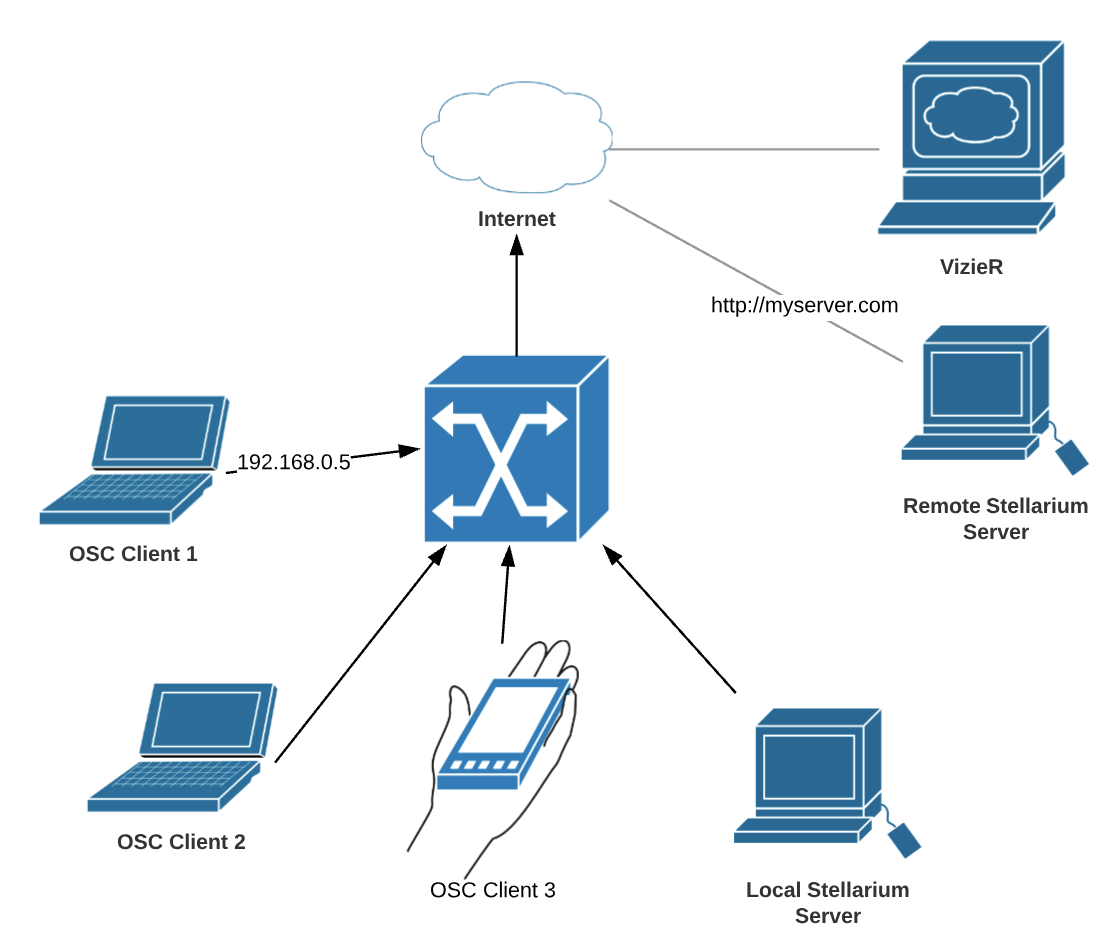
\includegraphics[width=1\columnwidth]{RemoteStellarium}
	\caption{Remote Stellarium and OSC Clients.}
	\label{fig:RemoteStellarium}
\end{figure}
\bigskip

Creating a connection between \textit{OSC Client 1} and \texttt{Remote Stellarium Server} is effected by adding adding the arguments \\\texttt{client=192.168.0.5} and \texttt{stellarium=http://myserver.com} to the command line.
This will cause the Stellar Command module to send OSC messages to ``192.168.0.5" and Stellarium commands to \textit{http://myserver.com} on HTP port 8090\footnote{The default Stellarium Remote Control port is 8090, however, this can be changed inside Stellarium. It is assumed that port forwarding when not using a local area network has been configured to send packages to the correct computer hosting Stellarium}, effectively acting as a proxy between the two.

   \begin{syntax}
	\medskip
	java -jar StellarCommand.jar port=1234 osc=/Stellar  {\char'134}\\client=192.168.0.5 stellarium=http://myserver.com\\
	\medskip
\end{syntax}
\bigskip

\clearpage
\pagestyle{ruled}

%#% extstart include laying-out-page.tex


\chapter{Using Stellar Command as a Java Library} \label{chap:libraryosc}
This chapter details how to use Stellar Command as a library that you call directly from within your programming environment.
If you intend to use Stellar Command as a standalone server application and communicate to it with Open Sound Control Messages through your preferred music package---such as Max MSP, SuperCollider or PD---you can skip back to chapter~\ref{chap:launchosc} --
\emph{\titleref{chap:launchosc}}.

    
\chapter{Comments}
\label{cha:comments}

\section{Algorithms}
\label{sec:algorithms}

Over time we may use this section to explain, or list some of the
algorithms for some of the macros in the class. The information may be
useful to some.

\subsection{Autoadjusting
  \texorpdfstring{\cs{marginparwidth}}{\textbackslash marginparwidth}}
\label{sec:auto-csmarg}

This algorithm is used within \cmd{\fixthelayout} unless the user have
used \cmd{\setmarginnotes}.

\noindent
\begin{framed}
  \vskip-2\baselineskip
  \begin{small}
\begin{verbatim}
if twocolumn then
  marginparwidth = min{inner margin,outer margin}
else
  if twoside then
    if marginpar always left or always right then
      marginparwidth = min{inner margin,outer margin}
    else if marginpar in outer margin then
      marginparwidth = outer margin
    else if marginpar in inner margin then
      marginparmargin = inner margin
    end if
  else
    if marginpar in left margin then
      marginparwidth = inner margin
    else
      marginparwidth = outer margin
    end if
  end if
end if
marginparwidth = marginparwidth - 2marginparsep
if marginparwidth < 1pt then
  marginparwidth = 1pt
end if
\end{verbatim}
  \end{small}
\end{framed}


%#% extend

%#% extstart input backend.tex


%%%%%%%%%%%%%%%%%%%%%%%%%%%%%%%%
%%\endinput
%%%%%%%%%%%%%%%%%%%%%%%%%%%%%%%

%%%%%%%%% end mbooka
%%%%%%%%%%%%%%%%%%%%%%%%%%%%%%%%%%%%%%%%%%%%%%%%%%%%%%%%%%%%

% back end
\backmatter

\PWnote{2009/07/08}{Changed \cs{toclevel@section} so that Notes 
                    divisions appear in the bookmarks}
\makeatletter\renewcommand*{\toclevel@chapter}{-1}\makeatother 
\makeatletter\renewcommand*{\toclevel@section}{0}\makeatother
\clearpage
\printpagenotes
\clearpage
\pagestyle{plainmarkruled}
%%\chapterstyle{section}

\renewcommand*{\begintheglossaryhook}{\small}
%%%\glossaryintoc
\printglossary

\renewcommand{\prebibhook}{%
\ctan\ is the \cTeXan. Information on how to
access CTAN is available at \url{http://www.tug.org}.
\par\vspace{\onelineskip}}

%%%\begin{comment}
\nocite{*}
\bibliographystyle{abbrv}

\bibliography{NIME_2019-planetarium} 


\clearpage
\twocolindex
\pagestyle{index}
%\renewcommand{\chaptermark}[1]{}
\renewcommand{\preindexhook}{%
The first page number is usually, but not always, the primary reference to
the indexed topic.\vskip\onelineskip}
\indexintoc

%%%\raggedright  does nasty things to index entries
\printindex

\onecolindex
\renewcommand*{\preindexhook}{}
\renewcommand*{\indexname}{Index of first lines}
%%% \indexintoc


\makeatletter
\renewcommand{\doidxbookmark}[1]{{\def\@tempa{Symbols}\def\@tempb{#1}%
  \centering\bfseries \ifx\@tempa\@tempb %
  Analphabetics 
%  \phantomsection%
%  \pdfbookmark[0]{Analphabetics}{Analphabetics-idx}%
%  \label{AnalphabeticsAnalphabeticsAnalphabetics-idx}%
  \else 
  #1%
%  \phantomsection%
%  \pdfbookmark[0]{#1}{#1-idx}%
%  \label{#1#1#1-idx}%
  \fi%
  \vskip\onelineskip\par}}
\makeatother


\printindex[lines]

\cleardoublepage
\pagestyle{empty}
\null\vfil

\begin{adjustwidth}{1in}{1in}
\begin{center}
{\Large\textsf{Colophon}}
\end{center}
\begin{center}
This manual was typeset using the \ltx\ typesetting system
created by Leslie Lamport and the \Mname\ class. 
The body text is set 10/12pt on a
33pc measure with Palatino designed by Hermann Zapf, which includes 
italics and small caps. Other fonts include
Sans, Slanted and Typewriter from Donald Knuth's 
Computer Modern family.

\end{center}


\end{adjustwidth}





\vfil

%#% extend


\end{document}

\endinput


%%% Local Variables: 
%%% mode: latex
%%% TeX-master: t
%%% TeX-source-specials-mode: t
%%% TeX-PDF-mode: t
%%% End: 
